\documentclass[runningheads]{llncs}

\usepackage[utf8]{inputenc}
\usepackage[ngerman]{babel}
\usepackage[T1]{fontenc}
\usepackage{amsmath}
\usepackage{amsfonts}
\usepackage{tikz}

\usepackage{graphicx}
\graphicspath{ {./images/} }

\usepackage{biblatex}
\addbibresource{referenzen.bib}
 
\title{Ensemble Clustering}
\subtitle{Seminar im Fachgebiet Wissensverarbeitung}

\author{Malek Alsalamat}
\institute{Universität Kassel}
\begin{document}

\maketitle	


  
\section{Was ist Clustering}
\textbf{Clustering} ist die Methode im maschinellen Lernen und genauer gesagt “im unüberwachten Lernen”, Datenpunkte in Gruppen (Clusters) ohne vorhandenes Wissen zu ordnen.  Um das zu schaffen, wird die Ähnlichkeit zwischen die Daten berechnet.\\[4pt]
Ziel von Clustering: 
\begin{itemize}
	\item Ähnliche Datenpunkte (Objekte) sollen im selben Cluster sein. 
	\item Datenpunkte im verschiedenen Cluster soll möglichst unähnlich sein.   
\end{itemize}
Also Clustering führt zu der Verringerung von der Komplexität.\\[4pt]
Die gefundenen Ähnlichkeitsgruppen können graphentheoretisch, hierarchisch, partitionierend oder optimierend sein. Inzwischen gibt es im Clustering eine große Vielfalt an Methoden, die eingesetzt werden können. Das hängt aber vom Anwendungsfall und der Größe der Datenmenge ab.\\[4pt]
Was man aber dabei beachten soll, dass die Algorithmen verschiedene Ergebnisse liefern können \cite{onlinequelle1}. 

\section{K-Means als Beispiel für partitionierende Verfahren}
Im partitionierenden Verfahren wird ein Clustering mit k Cluster mit minimalen Kosten gesucht. Und bei K-Means wie der Name bereits sagt, sucht das Algorithmus für jeden Cluster einen zentralen Punkt, bei dem die Varianz zu allen umliegenden Punkten möglichst gering ist.\\[4pt]
Das Ganze passiert in einem iterativen Verfahren wie folgendes \cite{onlinequelle1}:
\begin{itemize}
	\item Initialisierung: Zufällige Auswahl von K Zentren. 
	\item Zuweisung aller Datenpunkten zum nächstliegenden Zentrum, gemessen an einer Distanzmetrik. Distanzmetrik berechnet hier die Ähnlichkeit. 
	\item Verschieben der Zentren in den Mittelpunkt aller zugeteilten Datenpunkte.
	\item Gehe zu 2), außer ein Abbruchkriterium ist erreicht. Der Abbruchkriterium ist, wenn die Zentren sich nicht mehr ändern.    
\end{itemize}

\section{Ensemble Clustering}
Im Zusammenhang mit maschinellem Lernen ist Ensemble im Allgemein definiert als ein maschinelles Lernsystem, das mit einer Reihe von parallel arbeitenden einzelnen Modellen konstruiert wird. Und die Ergebnisse von diesen Modellen werden mit einer Entscheideungsfusionsstratigie kombiniert, um einzige Lösung für das gegebenen Problem zu liefern.\\[4pt]
 Die Ensemble Methode war zuerst nur im Bereich des überwachten Lernens benutzt und betrachtet, aber aufgrund seiner erfolgreichen Applikationen in Klassifizierungsaufgaben wurde es versucht, die Ensemble Methode auf unüberwachtes Lernen anzuwenden \cite{alqurashi2019clustering}. Insbesondere auf Clustering Probleme. Die Gründe dafür sind erstens, dass es kein vorhandenes Wissen über die zugrundeliegende Struktur. Zweitens es gibt keinen einzelnen Clustering-Algorithmus, der für verschiedene Probleme konsistent gute Leistungen erbringen kann.\\[4pt]
 Ensemble Clustering zielt darauf ab, mehrere Clusteringsmodelle zu kombinieren, um ein besseres Ergebnis als die einzelnen Clustering-Algorithmen. Dies ist in vielen Kontexten sehr nützlich \cite{strehl2002cluster}: 
\begin{itemize}
	\item Qualität und Robustheit  
	\item Knowledge Reuse 
	\item Distributed Computing     
\end{itemize}
Das Ensemble Clustering Problem lässt sich wie folgt beschreiben:\\[4pt]
\textbf{Gegeben}: Mehrere Clusterings aus verschiedenen Algorithmen von derselben Datenmenge.\\[4pt]
\textbf{Gesucht}: Ein kombiniertes Clustering, welches so viele Informationen wie möglich mit den gegebenen Clusterings teilt. 


\section{Das Ensemble Problem}
\textbf{Notation}: Sei $X$ = $\{x_1, x_2, \ldots, x_n\}$ eine Menge von Objekten (Datenpunkte). Eine Partitionierung dieser $n$ Objekten in $k$ Clusters kann als eine Menge von k Mengen von Objekten $\{C_{l} \mid l = 1, \ldots, k\}$ oder als ein Label Vektor $\lambda \in {N}^{n}$ dargestellt werden. Ein Clusterer $\Phi$ ist eine Funktion, welche einen Label Vektor bei gegebene Objekten liefert.\\[4pt] 
Eine Mengen von $r$ Clusterings (Labelings) $\lambda^{(1, \dots, r)}$ ist zu einem Clustering anhand einer Consensus Funktion kombiniert. 


\subsection{Beispiel}
Sei $X$ = $\{x_1, x_2, \ldots, x_7\}$ eine Menge von Objekte und 4 Clusters $\{C_{l}, C_{2}, C_{3}, C_{4}\}$. Die folgende Label Vektoren spezifizieren  vier Clusterings von $X$.\\[4pt]
$\lambda^{(1)}$ = $(C_{l}, C_{l}, C_{l}, C_{2}, C_{2}, C_{3}, C_{3})^{T}$ \qquad		
$\lambda^{(2)}$ = $(C_{2}, C_{2}, C_{2}, C_{3}, C_{3}, C_{l}, C_{l})^{T}$ \\
$\lambda^{(3)}$ = $(C_{l}, C_{l}, C_{2}, C_{2}, C_{3}, C_{3}, C_{3})^{T}$	\qquad
$\lambda^{(4)}$ = $(C_{l}, C_{2}, ?, C_{l}, C_{2}, ?, ?)^{T}$ \\[4pt]
$\lambda^{(1)}$ wird so gelesen: $x_1, x_2, x_3 \in C_{1}$ usw.\\
Man kann erkennen, dass die Label Vektoren $\lambda^{(1)}$ und $\lambda^{(2)}$ logischerweise identisch sind. $\lambda^{(3)}$ liefert einen Unterschied von der Zugehörigkeit der Objekte $x_3$ und $x_5$. $\lambda^{(4)}$ weicht sich von der Anderen sehr ab, außerdem $\lambda^{(4)}$ enthält $missing$ $Data$ \cite{strehl2002cluster}.\\
Gesucht ist jetzt ein kombiniertes Clustering, welches so viele Informationen wie möglich mit den vier gegebenen Clusterings teilt. Intuitiv, ein gutes kombiniertes Clustering in diesem Fall ist  $\lambda^{(1)}$ oder auch $\lambda^{(2)}$ .



\subsection{Objektive Funktion für Ensemble Clustering}
Gegeben nun $r$ Gruppierungen mit $\lambda^{(i)}$ ist die $i-te$ Gruppierung, welche $k^{i}$ Clusters hat. Eine $consensus$ Funktion ist wie folgt definiert $\Gamma:\mathbb{N}^{n \times r} \rightarrow \mathbb{N}^{n}$ \cite{strehl2002cluster}.
\begin{equation} 
\centerline{ $\Gamma$ : $\{\lambda^{i} \mid i \in {1, \ldots, r}\} \rightarrow \lambda$.}
\end{equation}
Wenn es grundsätzliche keine Informationen über die relative Bedeutung der einzelnen Gruppierungen gibt, dann ist eine sinnvolle Ziel für die $consensus$ Antwort, ein Clustering zu suchen, welches die meisten Informationen mit dem ursprünglichen \textbf{Clusterings} teilt.  \\
Im Folgenden brauchen wir zwei Definitionen und zwar von Entropie und gegenseitige Information.\\
\textbf{Entropie}: ist die minimale Beschreibungskomplexität einer Zufallsvariablen.\\
\textbf{Gegenseitige Information}: st die Kommunikationsrate im Gegenwart von Rauschen.\\
Gegenseitige Information, die ein symmetrisches Maß zur Quantifizierung der statistischen Informationen zwischen zwei Distributionen ist, liefert einen Hinweis auf die gemeinsame Informationen zwischen einem Paar von $Clusterings$. Seien $X$ und $Y$ zwei Zufallsvariablen beschrieben durch das Clustering $\lambda^{(a)}$ und $\lambda^{(b)}$ mit $k^{(a)}$ und $k^{(b)}$ Clusters. $I(X,Y)$ beschreibt die gegenseitige Information zwischen $X$ und $Y$, und $H(X)$ beschreibt die Entropie von $X$.\\
Zur Vereinfachung der Interpretation und Vergleichbarkeit ist eine normalisierte Version von $I(X,Y)$, welche zwischen 0 und 1 liegt, gewünscht. Dies folgt zur normalisierten gegenseitigen Information NMI \cite{strehl2002cluster}:
\begin{equation} 
\centerline{$NMI(X,Y) = \frac{I(X,Y)}{\sqrt{H(X)H(Y)}}.$}
\end{equation}
Da $I(X,Y)$ eine Metrik ist, also es gilt $I(X,Y) \leq min(H(X), H(Y))$, ist dann $NMI(X,X)$ = 1 genauso wie gewünscht.\\
Die zweite Gleichung kann durch von $Clusterings$ bereitgestellten Strichproben geschätzt werden. Sei $n_{h}^{(a)}$ die Anzahl von Objekten in Cluster $C_{h}$ anhand das Clustering $\lambda^{(a)}$ und $n_{l}^{(b)}$ die Anzahl von Objekten in Cluster $C_{l}$ anhand das Clustering $\lambda^{(b)}$. Sei $n_{h,l}$ die Anzahl der gemeinsamen Objekten zwischen Cluster $h$ anhand $\lambda^{(a)}$ und Cluster $l$ anhand $\lambda^{(b)}$. Dann ist \cite{strehl2002cluster}:
\begin{equation}
\centerline{$\phi^{(NMI)}(\lambda^{(a)}, \lambda^{(b)}) = \frac{\sum_{h=1}^{k^{(a)}} \sum_{l=1}^{k^{(b)}}n_{h,l} \cdot \log \biggl(\frac{n \cdot n_{h,l}}{n_{h}^{(a)} \cdot n_{l}^{(b)}} \biggr) }{\sqrt{\biggl(\sum_{h=1}^{k^{(a)}} n_{h}^{(a)} \log \frac{n_{h}^{(a)}}{n} \biggr)
			\biggl(\sum_{l=1}^{k^{(b)}} n_{l}^{(b)} \cdot \log \frac{n_{l}^{(b)}}{n} \biggr)}}.$}
\end{equation}
Von Gleichung $(3)$ wird einen Maß zwischen einer Menge $\Lambda$ und einem einzelnen Clustering $\hat{\lambda}$  als die durchschnittliche normalisierte gegenseitige Information definiert (ANMI) \cite{strehl2002cluster}: 
\begin{equation} 
	\centerline{$\phi^{(ANMI)}(\Lambda, \hat{\lambda}) = \frac{1}{r} \sum_{q=1}^{r} \phi^{(NMI)}(\hat{\lambda}, \lambda^{(q)}).$}
\end{equation}
Das optimale kombinierte Clustering $\lambda^{(k-opt)}$ ist das Clustering mit der maximalen durchschnittlichen gegenseitigen Information, wobei $k$ ist die Anzahl von $consensus$ Clusters. In anderen Worten, $\phi^{(ANMI)}$ ist unsere objektive Funktion und $\lambda^{(k-opt)}$ ist \cite{strehl2002cluster}:
\begin{equation} 
	\centerline{$\lambda^{(k-opt)} = \underset{\hat{\lambda}}{\arg\max} \sum_{q=1}^{r} \phi^{(NMI)}(\hat{\lambda}, \lambda^{(q)}),$}
\end{equation}
wobei $\hat{\lambda}$ durch alle mögliche $k-Partitionierungen$ läuft. \\  
In unserem Beispiel enthält das Clustering $\lambda^{(4)}$ $missing Data$. Für solche Fälle kann das objektive $consensus$ Clustering aus der Gleichung $(5)$ durch Berechnung eines gewichteten Durchschnitt von der gegenseitigen Information mit allen bekannten Clusters verallgemeinert werden \cite{strehl2002cluster}.   
\begin{equation} 
	\centerline{$\lambda^{(k-opt)} = \underset{\hat{\lambda}}{\arg\max} \sum_{q=1}^{r} \lvert \Upsilon^{(q)} \lvert \phi^{(NMI)}(\hat{\lambda}_{\Upsilon^{(q)}}, \hat{\lambda}_{\Upsilon^{(q)}}^{(q)}).$}
\end{equation}
Wobei $\Upsilon^{(i)}$ ist eine Menge von Indizes der Objekten mit bekannten Clusters für das $i-te$ Cluster. 



\section{Effiziente consensus Funktion}
In diesem Abschnitt werden einige Verfahren zur Lösung des Ensemble Clustering Problems vorgestellt. 
Es gibt zwei Arten von $consensus$ Funktionen, eine basiert auf die Median Partitionierung Approximation und die zweite basiert auf das gemeinsame Auftreten von Objekten, die sogenannte $objects$ $co-occurrence$ $approach$ \cite{vega2011survey}.\\
Eine Einordnung von der wichtigsten  $consensus$ Funktionen werden in $Abbildung 1$ vorgestellt. Aber wir werden uns hier nur auf die $Graph$ $and$ $hypergraph$ $based$ $methods$ fokussieren.
\begin{figure}[t]
	\begin{center}
		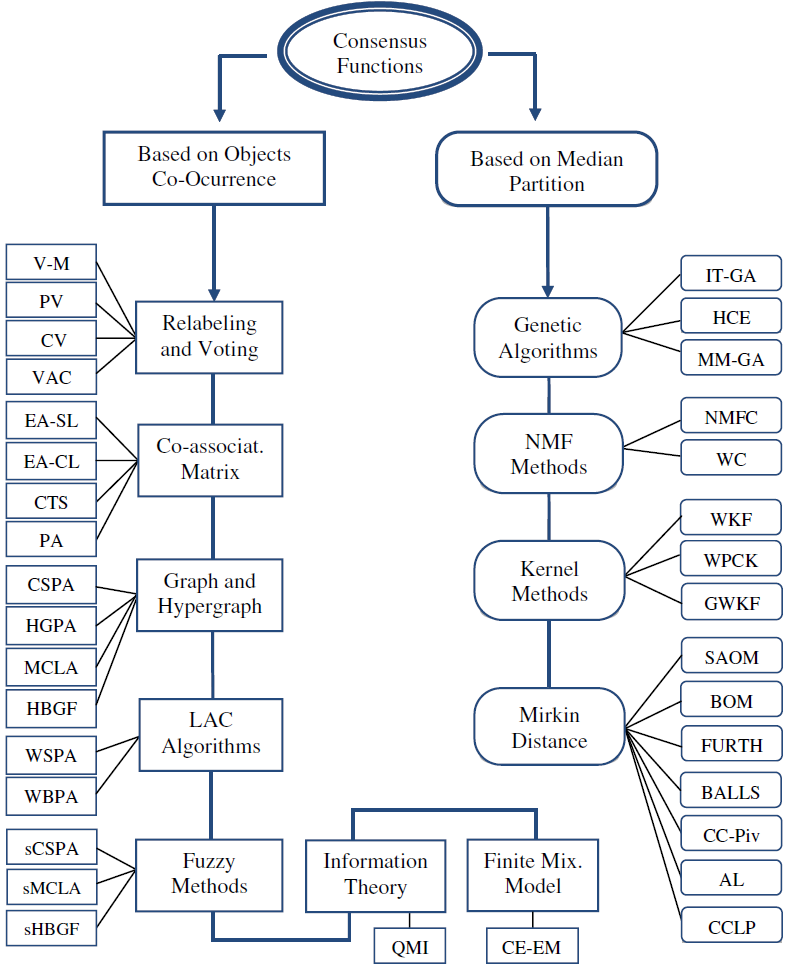
\includegraphics[width=10cm, height=10cm]{Abbildung1}
		\caption{Schematische Darstellung der wichtigsten Konsensfunktionstechniken. Konsensfunktionen, die auf dem Objekt
			objects co-occurrence approach basieren, sind durch ein Rechteck (links) dargestellt, die auf der Median Partitionierung Approximation werden durch ein abgerundetes Rechteck dargestellt (rechts) \cite{vega2011survey}.}
	\end{center}	
\end{figure}


\subsection{Graph and hypergraph based methods}
Diese Art von Clustering-Ensemble-Methoden transformieren das Kombinationsproblem zu einem Graph bzw. Hypergraph-Partitionierungsproblem. Der Unterschied zwischen den Methoden liegt auf die Art und Weise, wie der (Hyper-)Graph aus der Menge der Clusterings aufgebaut wird, und wie Kantenschnitt von der Graph definiert ist, um die $consensus$ Partitionierung zu erhalten.\\
Hier werden vier Methoden für diese Art von Clustering vorgestellt und zwar: 
\begin{itemize}
	\item Cluster-based Similarity Partitioning Algorithm (CSPA): Hier wird aus dem Hypergraph eine $n \times n$ Ähnlichkeitsmatrix (die Co-Assoziationsmatrix) konstruiert. Dies kann als eine Adjazenzmatrix eines zusammenhängenden Graphen angesehen werden, wobei die Knoten die Elemente der Datenmenge $X$ sind und die kanten zwischen zwei Objekten ein zugeordnetes Gewicht hat. Das Gewicht entspricht, wie oft sich die Objekte im selben Cluster befinden. Danach wird das Graph-Partitionierungsalgorithmus MEITS verwendet, um die $consensus$ Partitionierung zu erhalten \cite{vega2011survey}.\\[4pt]
	
	\item HyperGraphs Partitioning Algorithm (HGPA): Hier wird den Hypergraphen direkt partitioniert, indem die minimale Anzahl  von Hyperkanten eliminiert wird. Außerdem wird es davon ausgegangen, dass alle Hyperkanten das gleiche Gewicht haben. Und es wird nach der kleinstmöglichen Anzahl von Hyperkanten gesucht, die den Hypergraphen in $k$ zusammenhängende Komponenten von
	annähernd gleicher Dimension unterteilen. Für die Implementierung dieser Methode wird die Hypergraphs-Partitionierungspaket $HMETIS$ verwendet \cite{vega2011survey}.\\[4pt]
	
	\item  Meta-CLustering Algorithm (MCLA):Vor allem wird hier die Ähnlichkeit zwischen zwei Clusters $C_{i}$ und $C_{j}$ anhand des $Jaccard-Indexes$ bezüglich der Menge der Objekte definiert. Somit ist die Ähnlichkeitsmatrix zwischen Clusters gebildet, welche die Adjazenzmatrix des Graphen darstellt. Aber unter der Berücksichtigung, dass die Clusters als Knoten sind und der Kante zwischen zwei Knoten gewichtet ist, wobei das Gewicht die Ähnlichkeit zwischen Clusters entspricht. Danach wird dieser Graph mit dem METIS partitioniert und das erhaltene Cluster wird als Meta-Cluster bezeichnet.\\
	Schließlich, um die eindeutige Partitionierung zu finden, wird die Anzahl jedes Objektes im Meta-Cluster berechnet und jeder Objekt wird zu einem Meta-Cluster geordnet, in dem er öfter aufgetreten ist \cite{vega2011survey}.\\[4pt]
	      
	\item Hybrid Bipartite Graph Formulation (HBGF): In diesem letzten Algorithmus werden die Clusters und Objekten zusammen in derselben Graph modelliert. Bei dieser Methode wird der bipartite-Graph so gebildet, dass es keine Kanten zwischen Knoten gibt, falls sie beide entweder Objekte oder Clusters sind. Also es gibt nur Kanten zwischen zwei Knoten, falls ein Knoten einem Cluster repräsentiert und der Zweite einem Objekt, der zu diesem Cluster gehört, repräsentiert. Die $consensus$ Partitionierung wird unter der Verwendung von METIS oder $Spectral-Clustering$ erhalten \cite{vega2011survey}.  
\end{itemize}  


\subsection{Darstellung von Gruppen von Clusterings als Hypergraph}
Wie wir schon im vorherigen Abschnitt gesehen haben, die Clusterings sollten zu einem Hypergraph umgewandelt werden, damit eine der vier Methoden verwendet werden kann. Und das ist genau unser Ziel in diesem Abschnitt.\\
Ein \textbf{Hypergraph} besteht aus Knoten und Hyperkanten. Eine Kante in einem regulären Graph verbindet $genau$ zwei Knoten. Eine \textbf{Hyperkante} ist eine Verallgemeinerung einer Kante, da sie jede Menge von Knoten verbinden kann.\\[4pt]
Für jeden Label Vektor $(Clustering)$ $\lambda^{(q)} \in \mathbb{N}^{n}$ konstruieren wir die binäre Zugehörigkeitsindikatormatrix  $H^{(q)} \in \mathbb{N}^{n \times k^{(q)}}$, wobei jeder Cluster als Hyperkante $(Spalte)$ dargestellt wird (Siehe Abb.2). Alle Einträge einer Zeile in der binären Zugehörigkeitsindikatormatrix $H^{(q)}$ werden zu 1 addiert, falls die Zeile mit einem Objekt, welches sein Cluster bekannt ist, übereinstimmt. und Zeilen für Objekte mit unbekanntem Cluster sind mit Null ausgefüllt.\\
Die Blockmatrix $H = (H^{(1)} \ldots H^{(r)})$ definiert die Adjazenzmatrix eines Hypergraphen mit $n$ Knoten und $\sum_{q=1}^{r} k^{(q)}$ Hyperkanten. Jeder Spaltenvektor $\boldsymbol{h_{a}}$ spezifiziert eine Hyperkante $h_{a}$, wobei 1 anzeigt, dass der Knoten mit der entsprechenden Zeile zu der Hyperkante gehört und 0 gibt an, dass dies nicht der Fall ist. Somit haben wir jeder Cluster zu einem Hyperkante und die Menge von Clusterings zu einem Hypergraph abgebildet \cite{strehl2002cluster}.\\ 
\begin{figure}[t]
	\begin{center}
		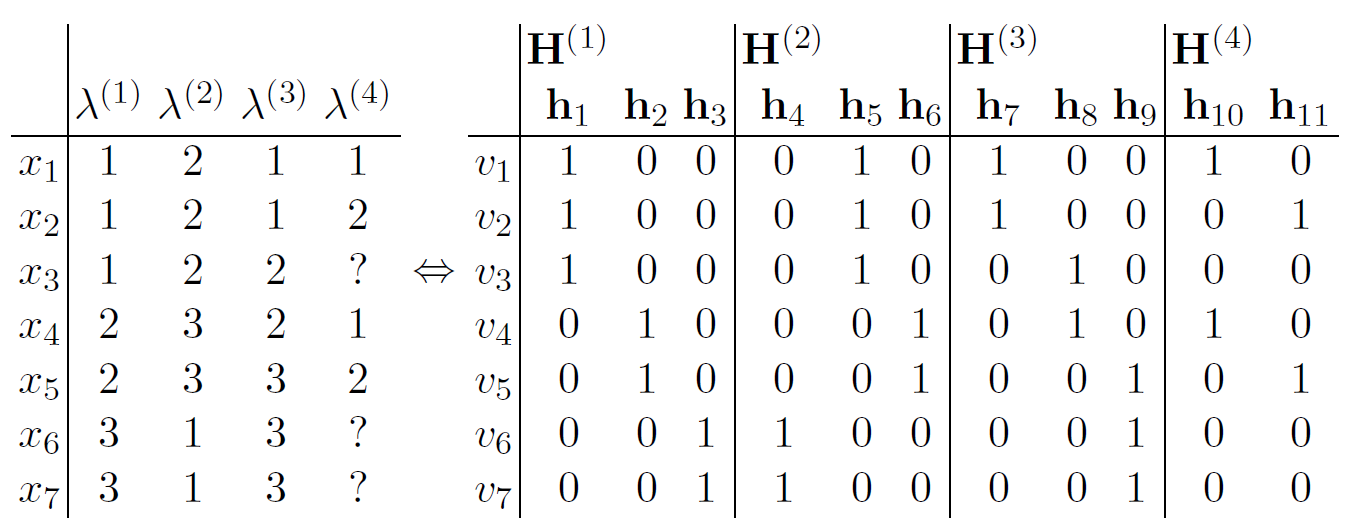
\includegraphics[width=\textwidth]{tablle1}
		\caption{Beispiel für das Cluster-Ensemble-Problem mit $r = 4$, $k^{(1, \ldots, 3)} = 3$ und $k^{(4)} = 2$: Original-Label-Vektoren (links) und äquivalente Hypergraphendarstellung mit 11 Hy-
			peredges (rechts). Jeder Cluster wird in eine Hyperedge umgewandelt \cite{strehl2002cluster}.}
	\end{center}	
\end{figure}


\section{Cluster-based Similarity Partitioning Algorithm}
In diesem Abschnitt wird das $Cluster-based$ $Similarity$ $Partitioning$ $Algorithm$ im Details geklärt. In diesem Algorithmus sollte zuerst eine Ähnlichkeitmatrix konstruiert werden. Basieren auf einer grob aufgelösten Suchtweise haben zwei Objekte eine Ähnlichkeit von $1$, falls sie im gleichen Cluster sind und eine Ähnlichkeit von $0$ ansonsten. Somit kann man eine $n \times n$ binäre Ähnlichkeitmatrix für jedes Clustering einfach erstellen. \\
Der eingangsbezogene Durchschnitt von $r$ solchen Matrizen, die die $r$ Gruppen darstellen, ergibt eine Gesamtähnlichkeitsmatrix S mit einer feineren Auflösung. Einträge von S bezeichnen den Anteil der Gruppierungen, in denen sich zwei Objekte im selben Cluster befinden,
und können mit einer einzigen dünnbesetzten Matrixmultiplikation $(sparse- matrix)$ berechnet werden S = $\frac{1}{r} H H^{T}$. Abb.3 veranschaulicht die Erstellung der clusterbasierten Ähnlichkeitsmatrix für das in Abb.2 angegebene Beispiel. Nun können wir die Ähnlichkeitsmatrix verwenden, um die Objekte mit einem beliebigen sinnvollen
Clustering-Algorithmus auf der Basis von Ähnlichkeit zu $reclustern$. In unserem Fall entscheiden wir uns für eine Partitionierung des induzierten Ähnlichkeitsgraphen (Knote = Objekt, Kantengewicht = Ähnlichkeit) mit METIS 
wegen seiner robusten und skalierbaren Eigenschaften.\\
CSPA ist die einfachste und naheliegendste Heuristik, aber ihr Rechen- und Speicheraufwand
Komplexität sind beide quadratisch in $O(n^2)$ \cite{strehl2002cluster}.
\begin{figure}[t]
	\begin{center}
		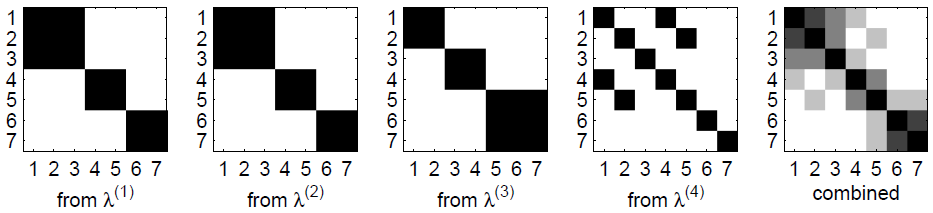
\includegraphics[width=\textwidth]{Abbildung2}
		\caption{Veranschaulichung von (CSPA) für das in Abb.2 angegebene Cluster-Ensemble-Beispielproblem. Jedes Clustering besitzt eine
			Ähnlichkeitsmatrix. Die Matrixeinträge werden durch Dunkelheit proportional zur Ähnlichkeit dargestellt.
			Ihr Durchschnitt wird dann verwendet, um die Objekte neu zu clustern und einen Konsens zu erhalten \cite{strehl2002cluster}.}
	\end{center}
\end{figure}


%\begin{center}
%	$r \cdot S$ = \quad
%	\begin{tabular}{  l| c c c c c c c}
%		\quad & $x_1$ & $x_2$ & $x_3$ & $x_4$ & $x_5$ & $x_6$ & $x_7$ \\ \hline 
%		$x_1$ & 4 & 3 & 2 & 1 & 0 & 0 & 0 \\
%		$x_2$ & 3 & 4 & 2 & 0 & 1 & 0 & 0 \\
%		$x_3$ & 2 & 2 & 3 & 1 & 0 & 0 & 0 \\
%		$x_4$ & 1 & 0 & 1 & 4 & 2 & 0 & 0 \\
%		$x_5$ & 0 & 1 & 2 & 4 & 1 & 1 & 1 \\
%		$x_6$ & 0 & 0 & 0 & 0 & 1 & 3 & 3 \\ 
%		$x_7$ & 0 & 0 & 0 & 0 & 1 & 3 & 3 \\
%	\end{tabular}
%\end{center}

\subsection{Mehrstufige Graphenbisektion}
Der Graph $G$ kann mit einem mehrstufigen Algorithmus halbiert werden. Die Grundstruktur eines mehrstufigen Algorithmus ist sehr einfach. Der
Graphen $G$ wird zunächst auf einige hundert Knoten runter vergröbert, dann wird eine Bisektion dieses viel kleineren Graphen berechnet und diese Partition dann auf den ursprünglichen Graphen zurückprojiziert Graph (feinerer Graph). Bei jedem Schritt der Entgröberung des Graphen wird die Partition weiter verfeinert. Solche Verfeinerungen verringern in der Regel den Kantenschnit ($edge-cut$).\\
Also Ein mehrstufiger Graphbisektionsalgorithmus funktioniert wie folgt: betrachte einen gewichteten Graphen $G_0 = (V_0, E_0)$ mit Gewichten sowohl aus Knoten als auch auf Kanten. Dieser Algorithmus besteht aus den folgenden frei Phasen \cite{karypis1998fast}:
\begin{itemize}
	\item Vergröberungsphase $Coarsening$: Der Graph $G_0$ wird in ein Folge von kleineren Graphen $G_1, G_2, \ldots, G_m$ umgewandelt, so dass $\lvert V_0 \lvert > \lvert V_1 \lvert > \ldots > \lvert V_m \lvert.$
	\item Partitionierungsphase: Eine 2-fache-Partition $P_m$ des Graphen $G_m = (V_m, E_m)$ wird berechnet, die $V_m$ in zwei Teile unterteilt, die jeweils die Hälfte der Knoten von $G_0$ enthält. 
	\item Entgröberungsphase $Uncoarsening$: Die Partition $P_m$ von $G_m$ wird auf $G_0$ zurückprojiziert, indem man durch die Zwischenpartitionen $P_{m-1}, P_{m-2}, \ldots, P_1, P_0$ geht.  
\end{itemize} 
\setcounter{secnumdepth}{3}
\subsubsection{Vergröberungsphase $(Coarsening)$}:\\[8pt]
In diesem Unterabschnitt beschreiben wir die grundlegende Ideen hinter der Vergröberung mit Hilfe von $Matchings$.\\
In den meisten Vergröberungsschemata wird eine Menge von Knoten von $G_i$ zu einem einzigen
Knoten des gröberen Graphen der nächsten Ebene $G_{i+1}$ kombiniert. 
Sei $V_{i}^{v}$ die Menge der Knoten von $G_i$, die zu einem Knoten $v$ von $G_{i+1}$ zusammengefasst wird. Wir werden $v$ als $Multi-Knote$ bezeichnen. Damit eine Bisektion eines gröberen Graphen in Bezug auf den ursprünglichen Graphen gut ist, wird das Gewicht des Knotens $v$ gleich der Summe der Gewichte der Knoten in $V_{i}^{v}$. Außerdem, um die Konnektivitätsinformationen im gröberen Graphen zu behalten, sind die Kanten von $v$ die Vereinigung der Kanten der Knoten in $V_{i}^{v}$. Für den Fall, dass mehr als ein Knoten von $V_{i}^{v}$ Kanten von demselben Knoten $u$ enthält, ist dann das Gewicht der Kante von $v$ gleich der Summe der Gewichte dieser Kanten. Dies ist nützlich, wenn wir die Qualität
einer Partition in einem gröberen Graphen bewerten wollen. Der Kantenschnitt der Partition in einem vergröberten Graphen
ist gleich dem Kantenschnitt der gleichen Partition in einem feineren Graphen.  \\
Bei einem Graphen $G_i = (V_i, E_i)$ kann man einen gröberen Graphen durch Kollabieren benachbarter Knoten erhalten. So wird die Kante zwischen zwei Knoten kollabiert und ein $Multi-Knote$
wird aus diesen beiden Knoten erstellt. Diese Idee von Kollabieren von Kanten lässt sich in Form von $Matching$ beschrieben werden. \\
Ein \textbf{Matching} eines Graphen ist eine Menge von Kanten, von denen keine zwei die auf denselben Knoten treffen. Der nächste gröbere Graph $G_{i+1}$ wird also aus $G_i$ konstruiert, indem ein $Matching$ von $G_i$ gefunden wird und die Knoten von diesem $Matching$ zu einem $Multi-Knote$ kollabieren. Alle Konten, die nicht im Matching waren, werden einfach im $G_{i+1}$ kopiert. Da das Ziel des Kollabieren von Knoten mit Hilfe von $Matching$ darin besteht, die Größe des Graphen $G_i$ zu verringern
, sollte das $Matching$ eine große Anzahl von Kanten enthalten. Aus diesem Grund werden $maximale$
$Matchings$ verwendet, um die aufeinanderfolgenden groben Graphen zu erhalten. Ein $Matching$ ist maximal
wenn jede Kante im Graphen, die nicht im Matching enthalten ist, mindestens einen ihrer Endknoten übereinstimmt.\\
 Beachten Sie, dass die Anzahl der Kanten, die zum maximalen Matching gehören, je nach Berechnungsmethode unterschiedlich sein kann. Das maximale Matching, das
die maximale Anzahl von Kanten hat, wird als $maximum$ $Matching$ genannt. Da jedoch die Komplexität der Berechnung eines $maximum$ $Matching$ im Allgemeinen höher ist als die Berechnung eines maximalen Matchings ist, werden letztere bevorzugt. Im verbleibenden Unterabschnitt beschreiben wir zwei Methoden, die wir zur Auswahl maximaler
Matchings für die Vergröberung. 
\begin{itemize}
	\item Random matching (RM): Ein maximales Matching kann mit einen randomisierten Algorithmus generiert werden. Die Knoten sind dann in  zufälliger Reihenfolge besucht. Wenn ein Knoten $u$ noch nicht ausgewählt wurde, dann wählen wir einen seiner nicht ausgewählter Nachbarknoten aus. Wenn es solcher Knoten $v$ existiert, wird die Kante $(u, v)$ zum Matching gefügt und markieren wir die Knoten $u$ und $v$ als besucht. Wenn es keinen solchen Konten $v$ gibt, dann bleibt $u$  wie es ist in der $RM$. Die Komplexität von diesem Algorithmus liegt in $O(\lvert E \lvert)$.\\[4pt]
	\item Heavy edge matching (HEM): $RM$ ist ein einfaches und effizientes Verfahren zur Berechnung einer
	maximale $Matching$ und minimiert die Anzahl der Vergröberungsstufen in einer gierigen Weise.
	Unser übergeordnetes Ziel ist es jedoch, eine Partition zu finden, die den Kantenschnitt $edge-cut$ minimiert.
	Betrachten wir
	einen Graphen $G_i = (V_i, E_i)$, ein Matching $M_i$, das zur Vergröberung von $G_i$ verwendet wird, und seinen gröberen Graphen
	$G_{i+1} = (V_{i+1}, E_{i+1})$, induziert durch $M_i$. Wenn A eine Menge von Kanten ist, so ist $W(A)$ die Summe
	der Gewichte der Kanten in A. Es kann gezeigt werden, dass
	\begin{equation} 
		\centerline{$W(E_{i+1}) = W(E_i) - W(M_i).$}
	\end{equation}
	Somit wird das Gesamtkantengewicht des gröberen Graphen um das Gewicht des $Matching$ verringert. Durch die Auswahl eines maximalen Matchings $M_i$, dessen Kanten ein großes Gewicht haben
	Gewicht haben, können wir das Kantengewicht des gröberen Graphen um einen größeren Betrag verringern. Da er ein geringeres Kantengewicht hat, auch einen kleineren Kantenschnitt. Die Suche nach einem maximalen $Matching$, das Kanten mit großem Gewicht enthält, ist die Idee hinter dem $HEM$.  Ein $HEM$ wird mit einem randomisierten Algorithmus berechnet, der dem zuvor beschriebenen Algorithmus zur Berechnung eines $RM$ ähnelt. Die Knoten werden wieder in zufälliger Reihenfolge besucht.\\
	 Anstatt jedoch einen Knoten $u$ zufällig mit einem seiner benachbarten nicht gematchten Knoten zu matchen, wird $u$ mit dem Knoten $v$ so gematcht, dass das Gewicht der Kante $(u, v)$ das Maximum über alle gültigen inzidenten Kanten ist (schwerere Kante). \\
	 Beachten Sie, dass dieser Algorithmus nicht garantiert, dass das erhaltene Matching ein maximales Gewicht (über
	 allen möglichen Matchings), aber im Allgemein funktioniert er sehr gut. Die Komplexität der Berechnung eines $HEM$ ist $O(\lvert E \lvert)$, was asymptotisch ähnlich ist zur Berechnung des $RM$.
\end{itemize}


\subsubsection{Partitionierungsphase}:\\[8pt]
Die zweite Phase eines Multilevel-Algorithmus berechnet
eine qualitativ hochwertige Bisektion (d. h. einen kleinen Kantenschnitt) $P_m$ des groben Graphen $G_m = (V_m, E_m)$,
so dass jeder Teil ungefähr die Hälfte des Knotengewichts des ursprünglichen Graphen enthält. Da bei der Vergröberung die Gewichte der Knoten und Kanten des vergröberten Graphen so eingestellt ist, dass sie die Gewichte der Knoten und Kanten des feineren Graphen widerspiegeln, enthält $G_m$ Informationen, um auf intelligente Weise die balancierte Partitionierung und die kleinen Kantenschnitt-Anforderungen durchzusetzen.\\
Eine Partition von $G_m$ kann mit verschiedenen Algorithmen erhalten werden, wie z.B \cite{karypis1998fast}:
\begin{itemize}
	\item spektrale Bisektion $SB$
	\item geometrische Bisektion (wenn Koordinaten verfügbar sind)
	\item kombinatorische Methoden
\end{itemize}
Da die Größe des
gröberen Graphen $G_m$ klein ist (d.h. $\lvert V_m \lvert < 100$), nimmt dieser Schritt nur wenig Zeit in Anspruch.
Es wird nur einen Algorithmus in diesem Abschnitt vorgestellt und zwar \textbf{Graph growing partitioning algorithm (GGP)}. Eine einfache Methode zur Bisektion des Graphen und sie funktioniert wir folgt:\\
Man startet bei einem beliebigen Knoten und bildet eine Region um ihn herum, bis die Hälfte der Knoten oder die Hälfte des gesamten Knotengewichtes einbezogen ist. Die Qualität des $GGP$ ist abhängig von der Wahl eines Knotens, von dem aus das Wachstum des Graphen beginnt, und verschiedene Startknoten ergeben unterschiedliche Kantenschnitte.  
 Um dieses Problem teilweise zu lösen, wählen wir zufällig 10 Eckpunkte
und lassen 10 verschiedene Regionen wachsen. Der Versuch mit dem kleineren Kantenschnitt wird als
die Partition ausgewählt. Diese Partition wird dann weiter verfeinert, indem sie als Eingabe für die $KL$.

\subsubsection{Entgröberungsphase $(Uncoarsening)$}:\\[8pt]
Während der Vergröberungsphase wird die Partition $P_m$ des vergröberten Graphen $G_m$ auf den ursprünglichen Graphen zurückprojiziert, indem man durch die Graphen $G_{m-1}, G_{m-2}, \ldots, G_1$ geht. Da jeder Knote con $G_{i+1}$ eine bestimmte Teilmenge von Knoten von $G_i$ enthält, erhält man $P_i$ aus $P_{i+1}$ durch einfaches Zuordnen der Menge der Knoten $V_{i}^{v}$, die mit $v \in G_{i+1}$ kollabiert sind, zu der Partition $P_{i+1}[v]$ (d.h $P_{i}[u] = P_{i+1}[v] \quad \forall u \in V_{i}^{v}$).   




\printbibliography


\end{document}